\section{Background and Notations}
\label{sec:background}

We start by introducing some of the notations we will be using throughout our manuscript (\cref{sec:notations}), followed by a review of JEPAs (\cref{sec:JEPA}), and existing literature studying their design (\cref{sec:mi}).


\subsection{Notations and Definitions}
\label{sec:notations}



\begin{figure*}[t!]
% \begin{figure*}[t!]
%     \centering
    \begin{definition}{JEPA}{}
    \begin{align}
    {\rm JEPA}(\vx) \iff& {\rm Enc}\left(\vx_{n,t+1,.}\right) \text { is predictable from }{\rm Enc}\left(\vx_{n,t,.}\right), \forall n,t\text{ and } {\rm Enc}\left(\vx_{.,.,.}\right) \text{ is not degenerate}.\label{def:SSL}
\end{align}
\begin{minipage}{0.32\linewidth}
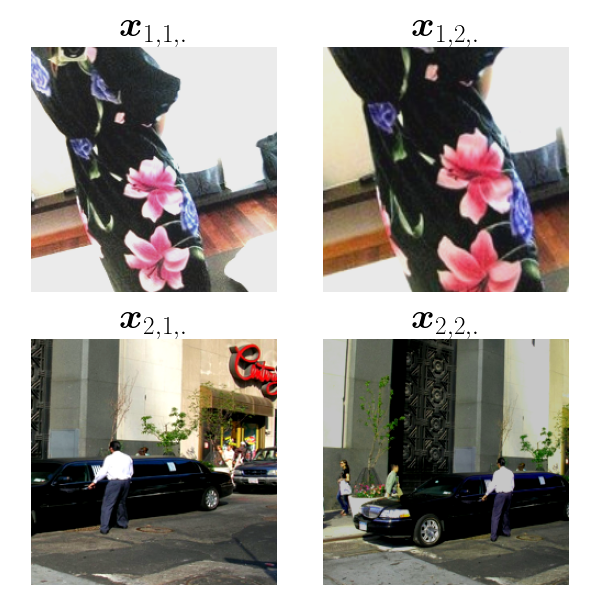
\includegraphics[width=\linewidth]{toy_figures/teaser/teaser_JEPA_0.png}
\end{minipage}
\begin{minipage}{0.32\linewidth}
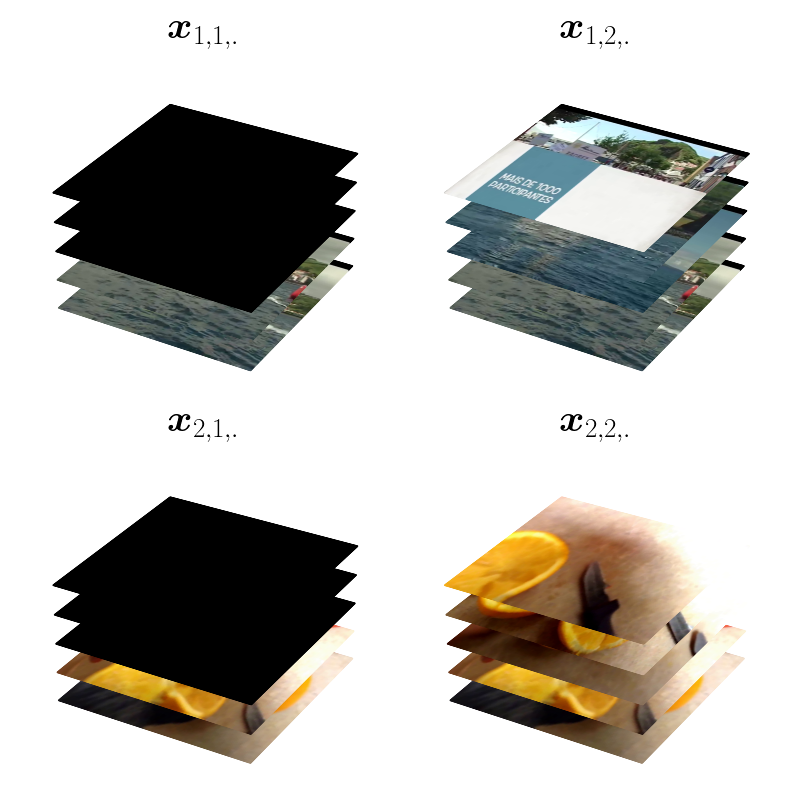
\includegraphics[width=\linewidth]{toy_figures/teaser/teaser_JEPA_1.png}
\end{minipage}
\begin{minipage}{0.32\linewidth}
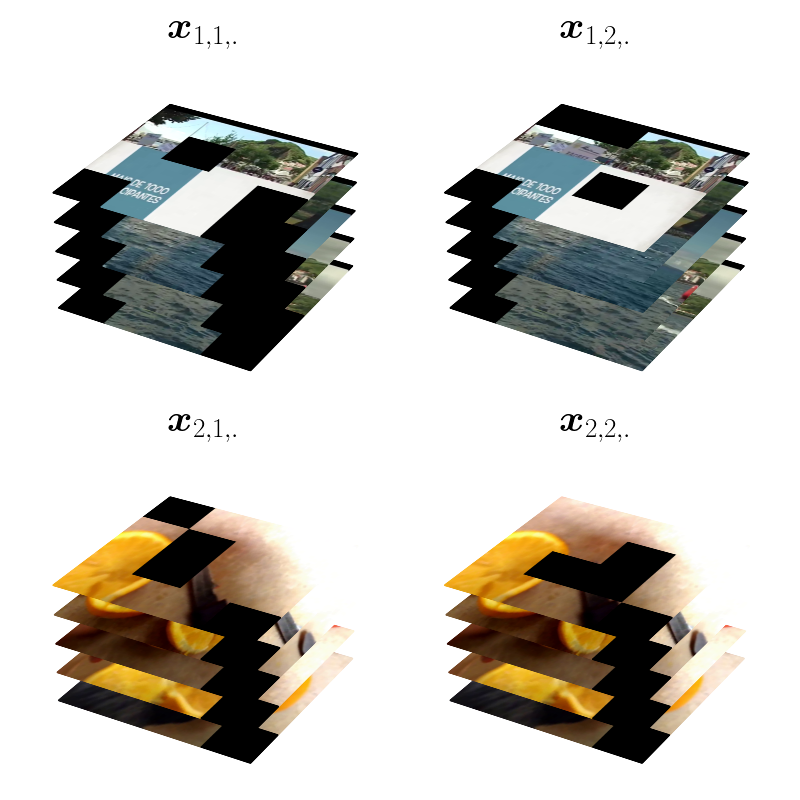
\includegraphics[width=\linewidth]{toy_figures/teaser/teaser_JEPA_2.png}
\end{minipage}
\end{definition}
\end{figure*}




{\bf Data.}~We are in possession of a dataset of shape $(N, V, D) \in {\mathbb{N}^*}^3$ where $N$ is the number of samples, $V$ is the number of views, and $D$ is the dimension. One entry of this dataset is accessed via $\vx_{n,v,d}$. Those dimensions are often interpreted as follows: ({\bf N}) is the number of independent samples, e.g., different images or different videos, ({\bf V}) is the number of {\em views}, e.g., data-augmentations for images, frames for videos, and ({\bf D}) is the dimension of each $\vx_{n,v}$, e.g., number of RGB pixels for images. In many cases the ordering over $V$ is given by {\em time}--but in some cases, e.g., data-augmentation of an image, ordering becomes irrelevant. Our study does not require any particular choice to organize one's dataset into a $(N,V,D)$ tensor--{\em and none of our theory and implementation assumes a particular design decision for that tensor}. However, we will rely on the following two properties, ({\em independence}) the samples $\vx_{n},\vx_{n'}$ have been obtained independently from each other $\forall n\not = n'$, and ({\em identically distributed}) the sampling process was identical among $\vx_{n}, \forall n$.

{\bf Deep Networks.}~Today's AI solutions rely on {\em Deep (Neural) Networks} (DNs), which are compositions of a large number of parameterized linear and nonlinear operators.
We denote the DN's mapping as $f_\vtheta: \R^D \rightarrow \R^K$ with $K$ the dimension of the embedding space. The internals of $f_\vtheta$ are designed by the researcher to incorporate as much prior knowledge about the data as possible. The details of $f_\vtheta$ are irrelevant to our study--as we will see the proposed LeJEPA works out-of-the-box on any $f_\vtheta$. In any case, all the {\em learnable parameters} are gathered in the vector  $\vtheta \in \R^P$, with $P$ counting the total number of parameters. A central challenge in AI research is to design the right architecture and training objective so that $\vtheta$ can be learned from gradient descent to ultimately produce a useful system, or foundation model, $f_{\vtheta}$. 



{\bf JEPAs.}~A foundation model is any system, e.g., a DN, able to solve numerous downstream tasks without requiring any change in its internal parameters $\vtheta$. This is in sharp contrast with a supervised model that only considers its training task. JEPAs have formally been introduced by \citet{lecun2022path} as a vehicle to produce foundation models. The core building blocks of JEPAs rely on numerous well-established techniques such as siamese networks \citep{bromley1993signature} and predictive coding \citep{helmholtz1867handbook,bruner1949perception}. While the exact blueprint of JEPAs varies greatly between use-cases, they all rely on two core principles: (i) being able to predict the embedding of a view $\vx_{n,v}$ from the embedding of another view $\vx_{n,v'}, v' \not = v$, all while (ii) ensuring that the embeddings do not become degenerate. Concretely, once a JEPA is designed and trained, it should be able to solve numerous downstream tasks in zero or few shots. 
The JEPA objective function, along with some examples for $\vx$, is provided in \cref{def:SSL}. The {\em predictability} criterion can be done by directly comparing the embeddings of the partial views $Enc(\vx_{n,v,.})$ and $Enc(\vx_{n,v',.})$ with a metric, e.g., $\ell_p$. In some cases, an additional DN coined {\em Pred}, is employed to compare $Pred(Enc(\vx_{n,v,.}))$ against $Enc(\vx_{n,v',.})$--which is only justified when there exists an asymmetry between the information content of the different views, e.g., by conditioning the predictions on observed actions from robotics data \citep{khazatsky2024droid}. 



\subsection{The Need for Reliable Pretraining}
\label{sec:JEPA}


The JEPA's prediction task is designed based on a priori knowledge of the data. Its design is often quite natural since it is relatively intuitive to form $\vx$ so that its views share the relevant information content one hope to capture. On the other hand, the design of the ``anti-collapse'' criterion is much closer to a game of Whac-A-Mole. Today's designs rely on many different under-specified safeguards which are carefully combined in the hope that degenerate shortcut solutions are avoided during training. Such mechanisms include (i) feature whitening \citep{ermolov2021whitening,bardes2021vicreg}, (ii) negative samples \citep{chen2020simple,he2020momentum}, and (iii) asymmetric views and teacher-student networks with stop-gradient \citep{caron2021emerging,assran2023self}. Those mechanisms all suffer from at least two of the following limitations: (i) under-specification, i.e., the criteria can be minimized while embeddings are in a degenerate configuration, (ii) quadratic time and memory complexity with mini-batch size and/or embedding dimension, (iii) sensitivity to data distribution, hyperparameters, architecture, and (iv) lack of theoretical understanding and guarantees. 






\subsection{The Need for Actionable Theory}
\label{sec:mi}


For decades, the two major solutions for AI were supervised learning \citep{lecun2015deep} and learning by reconstruction \citep{rumelhart1986learning}--sometimes combined together, e.g., for semi-supervised learning \citep{kingma2014semi}. In supervised learning, the labels both ensure that semantically similar samples are close to each other in embedding space while preventing complete representation collapse. In particular, it is possible to measure the amount of collapse in supervised learning as a function of the number of classes \citep{papyan2020prevalence}. The reconstruction objective is similarly well suited to prevent representation collapse as the original input must be recovered from the embeddings, i.e., the embeddings must be as informative about the input as possible--up to some optional denoising tasks that users can setup as part of the training \citep{vincent2010stacked}.


Because supervised and reconstruction-based learning have been widely studied for decades, there exists a large body of work to explain and inform practical designs--as well as studying their limitations in producing foundation models \citep{balestriero2024learning,van2025joint}. This is not the case for the more recent JEPAs where empirical advances quickly outpace anyone hoping to delve into their inner workings. This dynamic led the community to focus on post-hoc theoretical justification of already found solutions \citep{liu2021self,shwartz2024compress,shwartz2022we,zhang2023matrix}. In most cases, those studies involve the {\em Mutual Information (MI)} \citep{shannon1948mathematical,cover1999elements} whose different bounds recover established methods \citep{gutmann2010noise,ma2018noise,oord2018representation,poole2019variational,hjelm2018learning,mcallester2020formal}. Because existing studies focus on explaining and interpreting already developed JEPAs, too little principled guidance and innovation has been brought forward. Instead, most of the recent empirical advances take the form of collecting larger dataset, scaling up pre-existing training recipes \citep{goyal2019scaling,chen2020big,oquab2023dinov2,fan2025scaling}, and deriving novel data curation processes \citep{vo2024automatic,kerdreux2025efficient}. 

In contrast, our goal in the following \cref{sec:gaussian,sec:bcs,sec:lejepa} will be to derive a novel JEPA solution from first principles, i.e., whose design relies on proved necessary conditions for optimality, and with a pretraining recipe that can finally reconcile exploratory research, scalability, and state-of-the-art performances.








\section{Latent Euclidean: Embeddings Should be Isotropic Gaussian}
\label{sec:gaussian}


We address a fundamental question: {\em which distribution should ${\rm Enc}(\vx)$ 
follow to minimize empirical risk on any downstream task?} We prove that the 
isotropic Gaussian is the unique optimal distribution for both linear 
(\cref{sec:linear_probing}) and nonlinear probing (\cref{sec:nonlinear_probing}), 
with geometric intuition provided in \cref{sec:le}. This theoretical result 
establishes the necessary design principle for our JEPA; \cref{sec:bcs} 
then provides the practical implementation to achieve it.


\subsection{Linear Probing}
\label{sec:linear_probing}


We begin by identifying the optimal distribution for $f_\vtheta$'s embeddings 
by analyzing linear probes--one of the most popular methods for frozen 
encoder evaluation. Specifically, we ask: \emph{which distribution for 
$f_\vtheta(\vx)$ would be most favorable for solving arbitrary downstream tasks, 
i.e., for any realization of targets $\vy$?}


Denote as $\mZ \in \mathbb{R}^{N \times K}$ the matrix of $N$ embeddings, each $K$-dimensional, from $f_{\vtheta}(\vx_n)$. The {\em unknown} corresponding labels are denoted as $\vy \in \mathbb{R}^{N}$. Without loss of generality, we consider univariate targets; the 
following analysis extends to multivariate targets. The linear probe minimizes the following least square problem \citep{bishop2006pattern}
\begin{equation}
\hat{\beta} = \underset{\beta \in \mathbb{R}^K}{\arg\min} \|\vy - \mZ\beta\|_2^2+\lambda \|\beta\|_2^2,\tag{OLS}\label{eq:OLS}
\end{equation}
where $\hat{\beta}$ is the optimal probe parameters, and $\lambda \geq 0$ is an hyperparameter controlling the Tikhonov regularizer strength \citep{bishop1995training,golub1999tikhonov}. Despite not knowing $\vy$, it is possible to describe the bias and variance of the estimator $\hat{\beta}$ as a function of the distribution of $\mZ$. Consider two embeddings with identical column spans $\mZ_{\rm aniso}, \mZ_{\rm iso}$. $\mZ_{\rm aniso}$'s covariance matrix eigenvalues are given by $\{\lambda_k\}_{k=1}^K$ with at least two distinct values, while $\mZ_{\rm iso}$'s covariance matrix eigenvalues are all equal to $\frac{1}{K}\sum_{k=1}^{K}\lambda_k$. Hence, the two candidate embeddings $\mZ_{\rm aniso}, \mZ_{\rm iso}$ capture the same intrinsic features and have same energy, but different geometries.



\begin{lemma}[label={thm:linear_probe_bias}]{Anisotropy amplifies bias}{}
Whenever $\lambda_K>\lambda_1$, there always exists a downstream task ($\vy$) for which $\mZ_{\rm aniso}$ produces a higher bias estimator than $\mZ_{\rm iso}$ for $\lambda>0$. (Proof in \cref{proof:linear_probe_bias}.)
\end{lemma}
\begin{lemma}[label={thm:linear_probe_variance}]{Anisotropy amplifies variance}{}
With $\lambda=0$, the total variance of $\hat{\beta}$ \eqref{eq:OLS} is minimized for $\mZ_{\rm iso}$ with
$\text{tr}(\text{Var}(\hat{\boldsymbol{\beta}}_{\text{aniso}})) > \text{tr}(\text{Var}(\hat{\boldsymbol{\beta}}_{\text{iso}}))$. (Proof in \cref{proof:linear_probe_variance}.)
\end{lemma}



From the above \cref{thm:linear_probe_variance,thm:linear_probe_bias} we obtain that the distribution of features must be isotropic. We now move to nonlinear probing where the standard Gaussian will emerge as the unique optimum.


\subsection{Nonlinear Probing}
\label{sec:nonlinear_probing}


To allow for more flexible evaluation of the pretrained encoder $f_{\vtheta}$, it has become increasingly common to work with a nonlinear probe. We analyze two widely-used nonlinear methods: radius-based k-NN \citep{taunk2019brief,sun2010adaptive,zhang2017efficient,abu2019effects} for 
its simplicity and kernel methods \citep{nadaraya1964estimating,watson1964smooth} for their theoretical tractability. 

As in \cref{sec:linear_probing}, we ask ourselves which distribution of embeddings would be preferable for a foundation model. We first define our prediction function. The training data consists of the $N$ embeddings along with their training labels $\{(\vz_n,\vy_{n})\}_{n=1}^{N}$. The prediction, using radius-based k-NN for a query vector $\vq$ is formed as
\begin{align}
\widehat{\vy}(\vq) := \frac{1}{|\mathcal{N}_{r_0}(\vq)|}\sum_{n \in \mathcal{N}_{r_0}(\vq)}\vy_n,
\tag{kNN}\label{eq:kNN}
\end{align}
where $\mathcal{N}_{r_0}(\vq) = \{n : \|\vz_n - \vq\| \le r_0\}$. The specific choice of radius $r_0$ controls how many neighbors predictions are averaged to form the query's prediction. The kernel's prediction at a query $\vq\in\mathbb{R}^K$ is given by
\begin{align}
\widehat \vy(\vq)\triangleq \frac{\sum_{n=1}^N K_h(\vq-\vz_n)\vy_n}{\sum_{n=1}^N K_h(\vq-\vz_n)}.\tag{Kernel}\label{eq:NW}
\end{align}


We search over all distributions of Z subject to a fixed total variance 
constraint, e.g., $\Tr(\Cov(\mZ)) = \kappa_1$ or $\|\Cov(\mZ)\|_F=\kappa_2$. The specific value 
of $\kappa$ does not affect the optimal distribution shape.
Following the same type of derivations as done in the linear regime--with the exception of some additional regularity conditions--we are able to precisely identify the isotropic Gaussian as the unique optimum to minimize bias as formalized below. 



\begin{theorem}[label={thm:nonlinear_optimal}]{isotropic Gaussian Optimality}{}
The integrated square bias (ISB) over query points is given by
\begin{align*}
\text{ISB}_{k\text{-NN}} =\frac{r_0^4}{(K+2)^2}\tau_g^2J(p)+O(r_0^4),&&\text{(k-NN)}\\
\text{ISB}_{\text{kernel}} \le \Big(\frac{h^2\mu_2(K)}{2}\Big)^2 \Big(2 B^2 + 8 L^2J(p)\Big)+o(h^4),&&\text{(kernel)}
\end{align*}
and among distributions with a scalar-based covariance constraint, the isotropic Gaussian  is the unique minimizer of the integrated square bias. (Proof in \cref{proof:knn_optimal,proof:kernel_optimal}.)
\end{theorem}


Numerous additional details and discussions on the regularity assumptions we employed are provided in \cref{sec:additional_nonlinear}.
Together, these results establish the isotropic Gaussian distribution as the optimal design to minimize the worst-case risk of a foundation model across downstream tasks.





% We rely on the radial $k$-NN variation that leverages a sample-dependent $k$--improving performance for non uniform distributions of samples \citep{sun2010adaptive,zhang2017efficient,abu2019effects}. 


% We denote the underlying embedding density as $p_{z}\in C^3$ with derivatives of order up to $3$ bounded, and finite Fisher information and covariance. This regularity condition is fulfilled by current encoders. The {\em unknown} labels come from the target function $\eta:\R^K\to\R$, assumed $C^2$. We handle classification tasks by setting $\eta(\vz)=\mathbb{P}(Y=1\mid \vz)$. The training consists of the $N$ embeddings along with their training labels $\{(\vz_n,\eta(\vz_n))\}_{n=1}^{N}$, where we will denote $\vy_{n}\triangleq \eta(\vz_n)$. The prediction for a query vector $\vq$ is formed as
% \begin{align}
% \widehat{\vy}(\vq)
% :=
% \frac{1}{\vy(\vq)}\sum_{n:\norm{\vz_{n}-\vq}\le r_0}\vy_n,\tag{kNN}\label{eq:kNN}
% \end{align}
% with $\vy(\vq)\triangleq\#\{n:\norm{\vz_{n}-\vq}\le r_0\}$ counting the number of samples within a $r$-radius ball around $\vq$. The radius $r$ controls how many neighbors predictions are averaged to form the query's prediction. As per the linear probing's \cref{thm:linear_probe_bias}, we can characterize the bias of the estimator \cref{eq:kNN} at a particular query point, as formalized below.




% \begin{lemma}[label={thm:knn_bias}]{k-NN Pointwise Bias}{}
% The \eqref{eq:kNN} estimator has bias at query $\vq$ given by
% \begin{multline*}
%     \mathrm{Bias}(\vq)=
% \frac{r_0^2}{d+2}\Big(\grad\eta(\vq)^\top\grad\log p_{z}(\vq)+\tfrac{1}{2}\Delta\eta(\vz)\Big)\\+o(r_0^2),
% \end{multline*}
% where the remainder $o(r_0^2)$ is uniform in $\vq$. (Proof in \cref{proof:knn_bias}.)
% \end{lemma}


% To obtain the integrated bias, i.e., over the distribution of query points, we consider the following two properties. First, the distribution of query points follow the training distribution, i.e., $\vq \sim p_{z}$, second, target function $\eta$ has gradient which is mean-zero and isotropic with $\E\big[\grad\eta(\vz)\grad\eta(\vz)^\top\big]=\tau_g^2I_d$ with $\tau_g^2\in(0,\infty)$
% uniformly in $\vz$. We also have any finite scalar-constraint on the covariance of the embeddings such as $\Tr(\Sigma)=c$ or $\|\Sigma\|_F=c$ for a finite constant $c$.



% \begin{theorem}[label={thm:knn_optimal}]{k-NN isotropic Gaussian Optimality}{}
% The integrated squared bias of \eqref{eq:kNN} satisfies
% \[
% \E_{\vz}\big[\mathrm{Bias}(\vz)^2\big]
% =
% \frac{r_0^4}{(K+2)^2}\tau_g^2J(p)\\+O(r_0^4),
% \]
% and the isotropic Gaussian  is the unique minimizer of the integrated square bias. (Proof in \cref{proof:knn_optimal}.)
% \end{theorem}

% As a result, we now have a unique minimizer for the optimal embedding density for both the linear and k-NN probes.














% \subsection{Kernel Probing}
% \label{sec:kernel_probing}


% As an alternative to \eqref{eq:kNN}, it is also common to leverage kernel methods, which we consider in this section.


% Consider a kernel $K:\mathbb{R}^K\to\mathbb{R}$ with the following standard properties
% \begin{align}
%     &\int_{\mathbb{R}^d} K(u)du=1,\tag{normalized}\\
%     &\int_{\mathbb{R}^d} uK(u)du=0,\tag{symmetric}\\
%     &\int_{\mathbb{R}^d} u u^\top K(u)du=\mu_2(K)I_d,\tag{isotropic}\\
%     &R(K)\triangleq\int_{\mathbb{R}^d} K(u)^2du<\infty,\tag{finite roughness}
% \end{align}
% for some $\mu_2(K)\in(0,\infty)$, some bandwidth $h>0$ and denoting $K_h(t)\triangleq h^{-d}K(t/h)$, we remind the reader that the Nadaraya-Watson estimator, introduced in \citet{nadaraya1964estimating,watson1964smooth}, at a query $\vq\in\mathbb{R}^d$ is
% \begin{align}
% \widehat \vy(\vq)\triangleq \frac{\sum_{n=1}^N K_h(\vq-\vx_n)\vy_n}{\sum_{n=1}^N K_h(\vq-\vx_n)}.\tag{NW}\label{eq:NW}
% \end{align}
% Similarly to \eqref{eq:kNN}, we will see that the performance of \eqref{eq:NW} depends crucially on the distribution of the training points. Using the notations of \cref{sec:knn_probing}, we have access to our dataset of inputs from $p_z$ and for each sample $\vz_n$ the corresponding target is given from $\eta(\vz_n)=\mathbb{E}[Y_n\mid \vz_n]$. We also denote the corresponding conditional variance of the target function at that point as $v(x)=\mathrm{Var}(Y_i\mid X_i=x)$. We follow the regularity conditions of \cref{sec:knn_probing} and additionally assume that $p$ has sufficiently light tails so that for each coordinate $j$, $\lim_{\|x\|\to\infty} p(x)=0$ and $\lim_{\|x\|\to\infty} x_jp(x)=0$. We first derive the pointwise bias and variance for $\widehat \vy(\vq)$.


% \begin{lemma}[label={thm:kernel_bias}]{Kernel Bias and Variance}{}
% For any fixed $\vq\in\mathbb{R}^d$ with $p(\vq)>0$, as $h\to 0$ and $n h^d\to\infty$,
% \begin{align*}
% \mathrm{Bias}\big[\widehat \vy(\vq)\big]
% &=\frac{h^2\mu_2(K)}{2}\Big(\Delta \vy(\vq)+2\nabla \vy(\vq)^\top \nabla\log p(\vq)\Big)+o(h^2),\\
% \mathrm{Var}\big[\widehat \vy(\vq)\big]
% &=\frac{R(K)}{n h^d}\frac{v(\vq)}{p(\vq)}+o\big((n h^d)^{-1}\big).
% \end{align*}
% The $o(\cdot)$ terms are uniform over compact sets where $p$ is bounded away from zero.
% (Proof in \cref{proof:kernel_bias}.)
% \end{lemma}



% We now show that, under a fixed mean and total-covariance constraint on $p_z$, the isotropic Gaussian distribution uniquely minimizes the bias and variance of the kernel regression estimator at any test point. We restrict the smoothness class of the target function using 
% \begin{multline*}
%     \mathcal{M}(L,B)\triangleq\Big\{m\in C^2(\mathbb{R}^d):\|\nabla \vy(\vq)\|\le L,\\|\Delta \vy(\vq)|\le B, \forall  \vq\in\mathbb{R}^d\Big\},
% \end{multline*}
% allowing us to formalize below the worst case integrated bias and the optimal density for $z$.



% \begin{theorem}[label={thm:kernel_optimal}]{Kernel isotropic Gaussian Optimality}{thm:kernel_optimal}
% The integrated squared bias of \eqref{eq:NW} satisfies
% \begin{multline*}
% \sup_{m\in\mathcal{M}(L,B)}\mathbb{E}_{z}\left[\mathrm{Bias}\big[\widehat \vy(\vz)\big]\right]
% \le \Big(\frac{h^2\mu_2(K)}{2}\Big)^2\\\times \Big(2 B^2 + 8 L^2J(p)\Big)+o(h^4),
% \end{multline*}
% and the integrated variance is independent of $p$. 
% Among all densities $p$ on $\mathbb{R}^d$ with total-variance constrained, e.g., $\Tr(\Sigma)=c$, the isotropic Gaussian is the unique minimizer. (Proof in \cref{proof:kernel_optimal}.)
% \end{theorem}
